%%%%%%%%%%%%%%%%%%%%% chapter.tex %%%%%%%%%%%%%%%%%%%%%%%%%%%%%%%%%
%
% sample chapter
%
% Use this file as a template for your own input.
%
%%%%%%%%%%%%%%%%%%%%%%%% Springer-Verlag %%%%%%%%%%%%%%%%%%%%%%%%%%

\chapter{Processor Allocation and Process Migration}

\section{Problems and Goals}
\paragraph{Scheduling a System}
The discussion involves
\begin{itemize}
    \item pick a processor to run a process
    \item move a process from one processor to another processor
\end{itemize}

\paragraph{Process Migration}
The discussion involves
\begin{itemize}
    \item decide a process that should be migrated.
    \item select a new host for the process
    \item migrate the resource of the process
\end{itemize}

The migration here is talking about process. The threads of one process should be migrated together. We do not discuss that the threads are dispatched on different processors.

\section{Processor Allocation}
You need to be careful when you want to migrate a process. There is a difference between \emph{remote execution} and \emph{processor allocation}. People may not know that their local processes have been migrated to a remote processor and executed remotely.

\subsection{Approaches}

\subsubsection{A Centralized Approach: Up-Down}
There are CPU consumers and suppliers existing in the network. We give credits to the suppliers and take credits from the consumers. The hosts with more credits can have high probability to acquire a CPU.

\subsubsection{Hierarchical Approach}
\paragraph{Goal}
Hierarchical Approach can reduce the communication and information across the network in order to balance the load. 

\paragraph{Method}
There are workers on the leaves, and managers on the inner nodes. If a worker gets too much work or too little work, it will inform the manager above.
\begin{itemize}
    \item The manager will use the information to try a shift between workers of it.
    \item The manager meets the limit of its quotas, then tell the directors who try to balance the load among the managers.
\end{itemize}

\begin{figure}
\centering
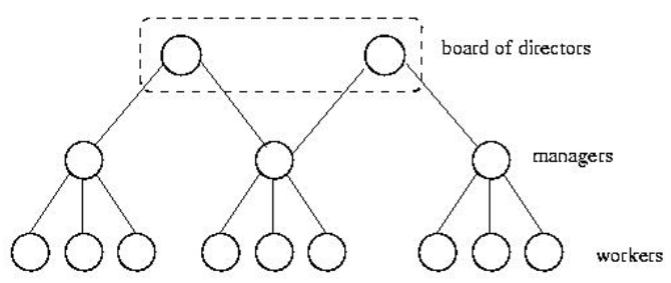
\includegraphics[width=\textwidth]{img/ch02-hier_proc.png}
\caption{Hierarchical Processor Management}
\label{fig:ch02-hier_proc}
\end{figure}

\paragraph{Loads}
We discussed the method for balance loads above that the workers gets too much work or too little work, it will inform managers. But how it communicate the information with managers and workers.

\begin{enumerate}
    \item Yell out. When a worker meets the situation, it yells out to others. If it is idle, it may cause \emph{thundering herds} that everyone wants to use it which makes it busy immediately.
    \item Receiver Initiated. The idle processor asks around. But this approach leads to heavy communications.
    \item Sender Initiated. The busy processor asks around to reduce load.
    \item Hybrid Approach. These try to balance the costs of the above two approaches. They only "yell out" if they are substantially overworked or under worked.
\end{enumerate}

\section{Process Behavior and Scheduling}
In general-purpose systems, recently started jobs are likely to be short lived, whereas long-running jobs are likely to keep running for a very long time.

\section{Process Migration}
Some ideas are here:
\begin{itemize}
    \item Virtual Machine can make the migration easier, but it arises some network problems, such as IP address.
    \item If we want to migrate processes, we need to build a recoverable, portable communication layer (do not hack with TCP). This layer allows suspend, update and resume programs.
    \item There are some systems working for this scheduling: HTCondor, TORQUE.
\end{itemize}